% Options for packages loaded elsewhere
\PassOptionsToPackage{unicode}{hyperref}
\PassOptionsToPackage{hyphens}{url}
%
\documentclass{article}
\usepackage{polski}
\usepackage{lmodern}
\usepackage{hyperref}
\usepackage{amssymb,amsmath}
\usepackage{ifxetex,ifluatex}
\usepackage{amssymb}
\usepackage{cite}
\usepackage{listings}
\usepackage{float}
\usepackage{subfig}
\usepackage{color}
\usepackage{amsmath}
\setcounter{tocdepth}{3}
\usepackage{graphicx}
\usepackage{amssymb}
\usepackage[a4paper]{geometry}
\usepackage[T1]{fontenc}
\usepackage{color}
\usepackage{url}
\usepackage[dvipsnames]{xcolor}
\usepackage{hyperref}
\hypersetup{
    colorlinks=true,
    linkcolor=violet,
    filecolor=magenta,      
    citecolor=blue,
    urlcolor=cyan,
}
\usepackage{graphicx}
\usepackage{mathtools}

\DeclarePairedDelimiter\ceil{\lceil}{\rceil}
\DeclareMathOperator*{\argmin}{argmin}
\DeclarePairedDelimiter\floor{\lfloor}{\rfloor}


\newcommand{\wek}[1]{
	{\bf{#1}} 
}
\newcommand{\jed}[1]{
	{$\left[#1\right]$}
}
\newcommand{\ma}[1]{
	{\bf #1} 
}
\newcommand{\todo}[1]{
	\colorbox{yellow} {{\color{red}
	\emph {TODO: #1}
}}}
\newcommand{\srednia}[1]{
	\langle #1 \rangle 
}




\title{Analiza metod detekcji anomalii na podstawie przebiegu kursów
instrumentów finansowych}
\author{Aleksandra Dzieniszewska \and Eryk Warchulski}
\date{}

\begin{document}
\maketitle
\begin{abstract}
  Celem niniejszego dokumentu jest przedstawienie wstępnych założeń
  dotyczących realizacji projektu analizy algorytmów detekcji anomalii w
  szeregach czasowych, tj. TSAD (z ang. \textbf{time series anomaly
  detection}). W jego ramach zostanie omówiona domena problemu, tj.
  przebiegi wartości instrumentów finansowych na różnych typach rynków,
  model zjawiska detekcji anomalii oraz plan eksperymentów. Opisane
  zostaną również metryki jakości uzyskiwanych rozwiązań jak i źródło
  pozyskiwanych danych.
\end{abstract}

\section{Wprowadzenie}

  Przebieg kursów aktywów finansowych jak na przykład kursów akcji
  spółek lub indeksów giełdowych jest fundamentem działania inwestorów na
  rynkach. Jego zachowanie determinuje strategie oraz ryzyko inwestycyjne.
  W związku z powyższym  kursy akcji są szczególnie interesujące nie
  tylko dla bezpośrednich aktorów rynkowych, ale również ekonomistów lub
  statystyków, którzy opracowują modele zachowań tych kursów lub rynków w
  ogólności. Współcześnie bardzo dużo uwagi poświęca się zagadnieniom
  predykcji przyszłych wartości kursów, co stanowi złożony i trudny
  problem, biorąc pod uwagę fakt, że jedna z dominujących teorii
  rynkowych, tj. EFM (z ang. \textbf{efficient-market hypothesis}) uważa
  za niemożliwe dokonywanie przydatnych predykcji \cite{RandomWalk}
  przyszłych kursów, a ponadto uznaje się, że rynki finansowe nie są
  obojętne na predykcje jak np. pogoda \cite{Sapiens}. Niemniej jednak
  problem predykcji przyszłych wartości kursów nie jest jedynym
  zagadnieniem, które ma praktyczne znaczenie. Możliwość odróżnienia
  niestandardowych fluktuacji kursów i tym samym punktów odstających może
  stanowić istotną informację dla inwestorów i zaangażować dedykowane
  takim zdarzeniom procesy biznesowe. Szczególnie istotne wydaje się to z
  punktu widzenia zautomatyzowanych rynków giełdowych, w których akcje
  podejmowane przez aktorów (systemy decyzyjne) mierzone są w
  milisekundach, a dane giełdowe mogą być traktowane jako strumieniowe
  \cite{HFT-wiki}. Wówczas wykrycie anomalii i jej odpowiednie obsłużenie
  wydaje się być krytyczne dla gracza rynkowego.
  \newline
  

  \section{Rynki finansowe \label{r2}}

  W ramach realizacji projektu użyte zostaną łącznie dwa zbiory danych, na
  które składają się przebiegi kursów instrumentów finansowych. Jeden z
  nich będzie pochodzić z rzeczywistego rynku finansowego, a drugi z rynku
  wirtualnego. Motywacją takiego podejścia jest chęć zaobserwowania
  zachowania się rynku w świecie, w którym na wartość kursu wpływa bardzo
  duża liczba czynników jawnych lub niejawnych, oraz w świecie, w którym
  zbiór możliwych akcji podejmowanych przez aktorów jest znacząco
  ograniczony oraz sam świat ma raczej charakter statyczny i iteracyjny.
  Ponadto dodatkową motywacją za skorzystaniem z danych pochodzących z
  rynku wirtualnego jest łatwość określenia zdarzeń, które powodują nagłe
  zmiany przebiegu kursu -- co zostanie bardziej szczegółowo opisane w
  podsekcji poświęconej temu rynkowi.

\subsection{Rynki rzeczywiste}

  \emph{Indeks giełdowy WIG20} jest statystyką (średnia ważona
  kapitalizacją spółek) obrazującą zmianę cen akcji dwudziestu
  największych spółek akcyjnych notowanych na Warszawskiej Giełdzie
  Papierów Wartościowych. Wartość indeksu pozwala ocenić inwestorom ogólny
  kierunek zmian cen i stan rynku.

  Przebieg indeksu WIG20 w wybranym przedziale czasowym pokazany jest na
  rysunku poniżej.

\begin{figure}
    \centering
    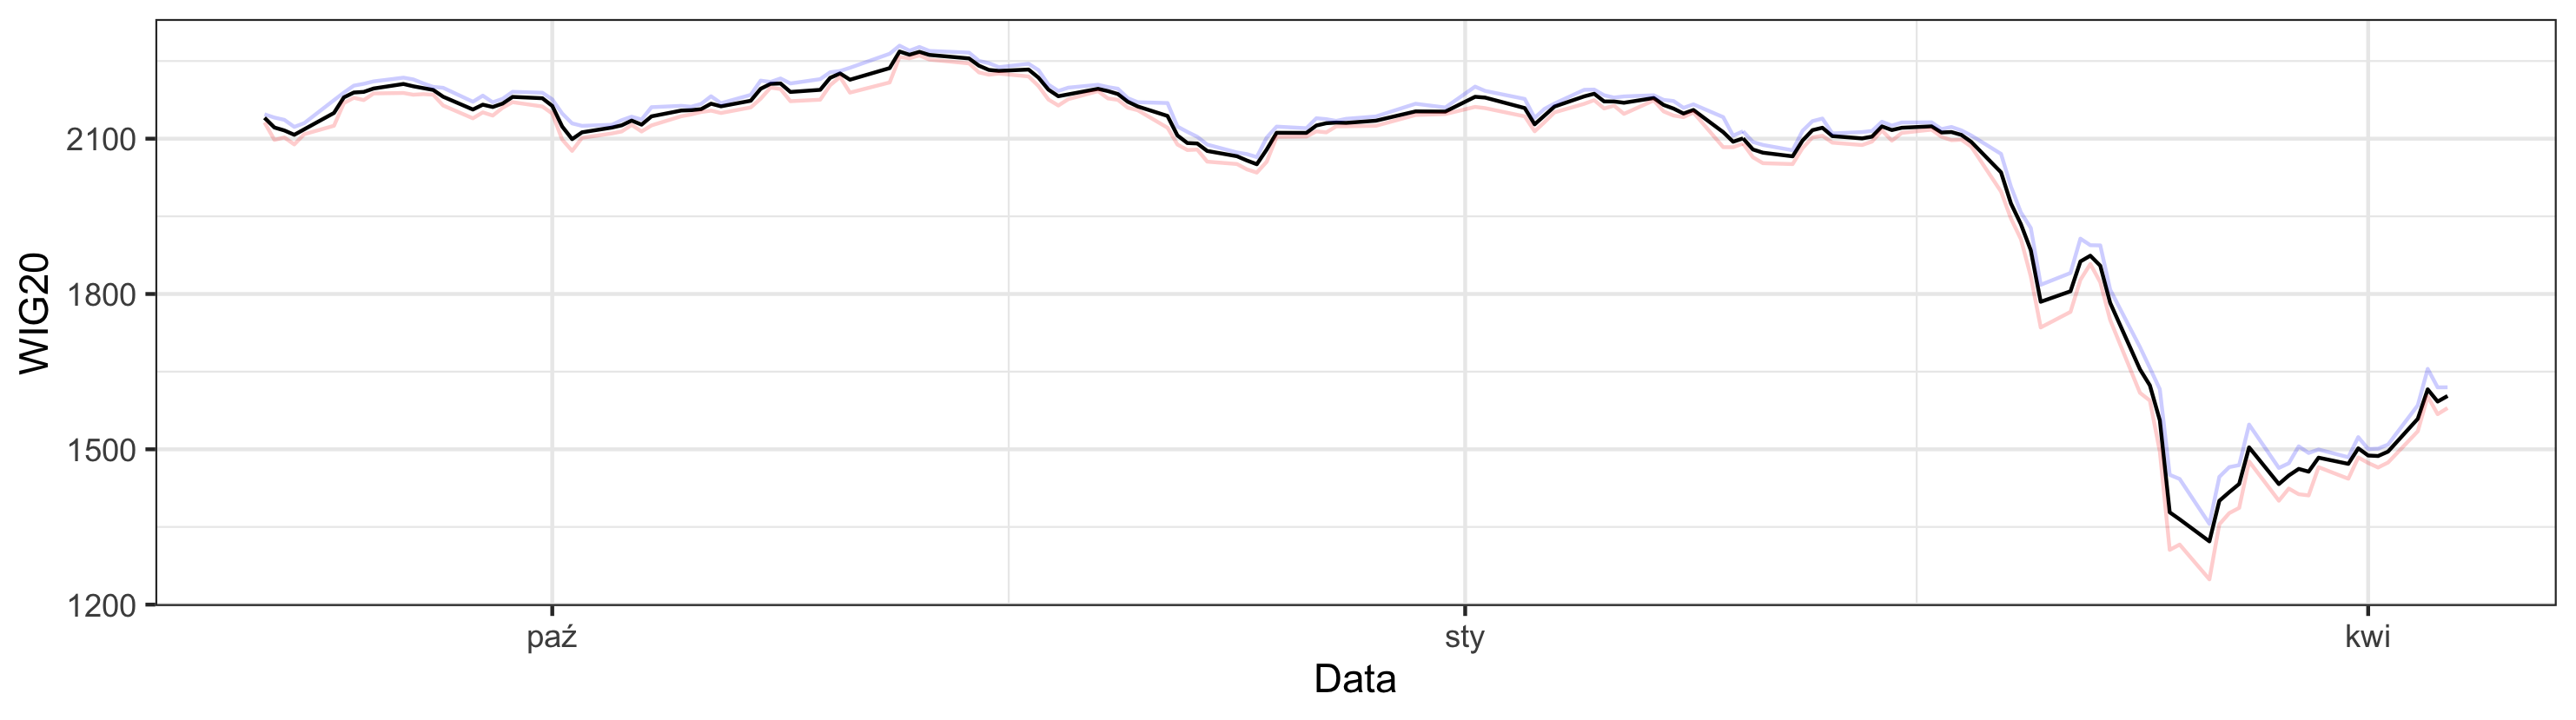
\includegraphics[width=\textwidth]{./images/wig20-random.png}
    \caption{Przebieg indeksu giełdowego WIG20. Rysunek własny.}
\end{figure}
\subsection{Rynki wirtualne}

\emph{WoW Token} jest przedmiotem w grze MMO-RPG (\emph{Massively
multiplayer online role-playing game}) \emph{World of Warcraft}, który
przez gracza może zostać wykorzystany w następujące sposoby:

\begin{itemize}
\item
  gracz może kupić token za rzeczywistą walutę (USD, GBP, EUR, TWD,
  KRW), a następnie sprzedać go w umieszczonym w grze domu aukcyjnym
  (\emph{Auction House})
\item
  gracz może kupić token, płacąc fikcyjną walutą obowiązującą w świecie
  \emph{World of Warcraft} (dalej G), a następnie wymienić go na
  przedłużenie abonamentu gry lub wymienić go na bon w internetowym
  sklepie wydawcy gry.
\end{itemize}

Kurs wymiany G/USD jest stały i wynosi $20$ \footnote{To samo tyczy
  się jakiejkolwiek innej waluty rzeczywistej.} natomiast kurs tokena w
świecie gry jest zmienny i zależy głównie od podaży i popytu
\cite{wtoken-info}.

Przebieg ceny tokena w grze na serwerach europejskich w wybranym czasie
jest pokazany na poniższym rysunku.

\begin{figure}
  \centering
  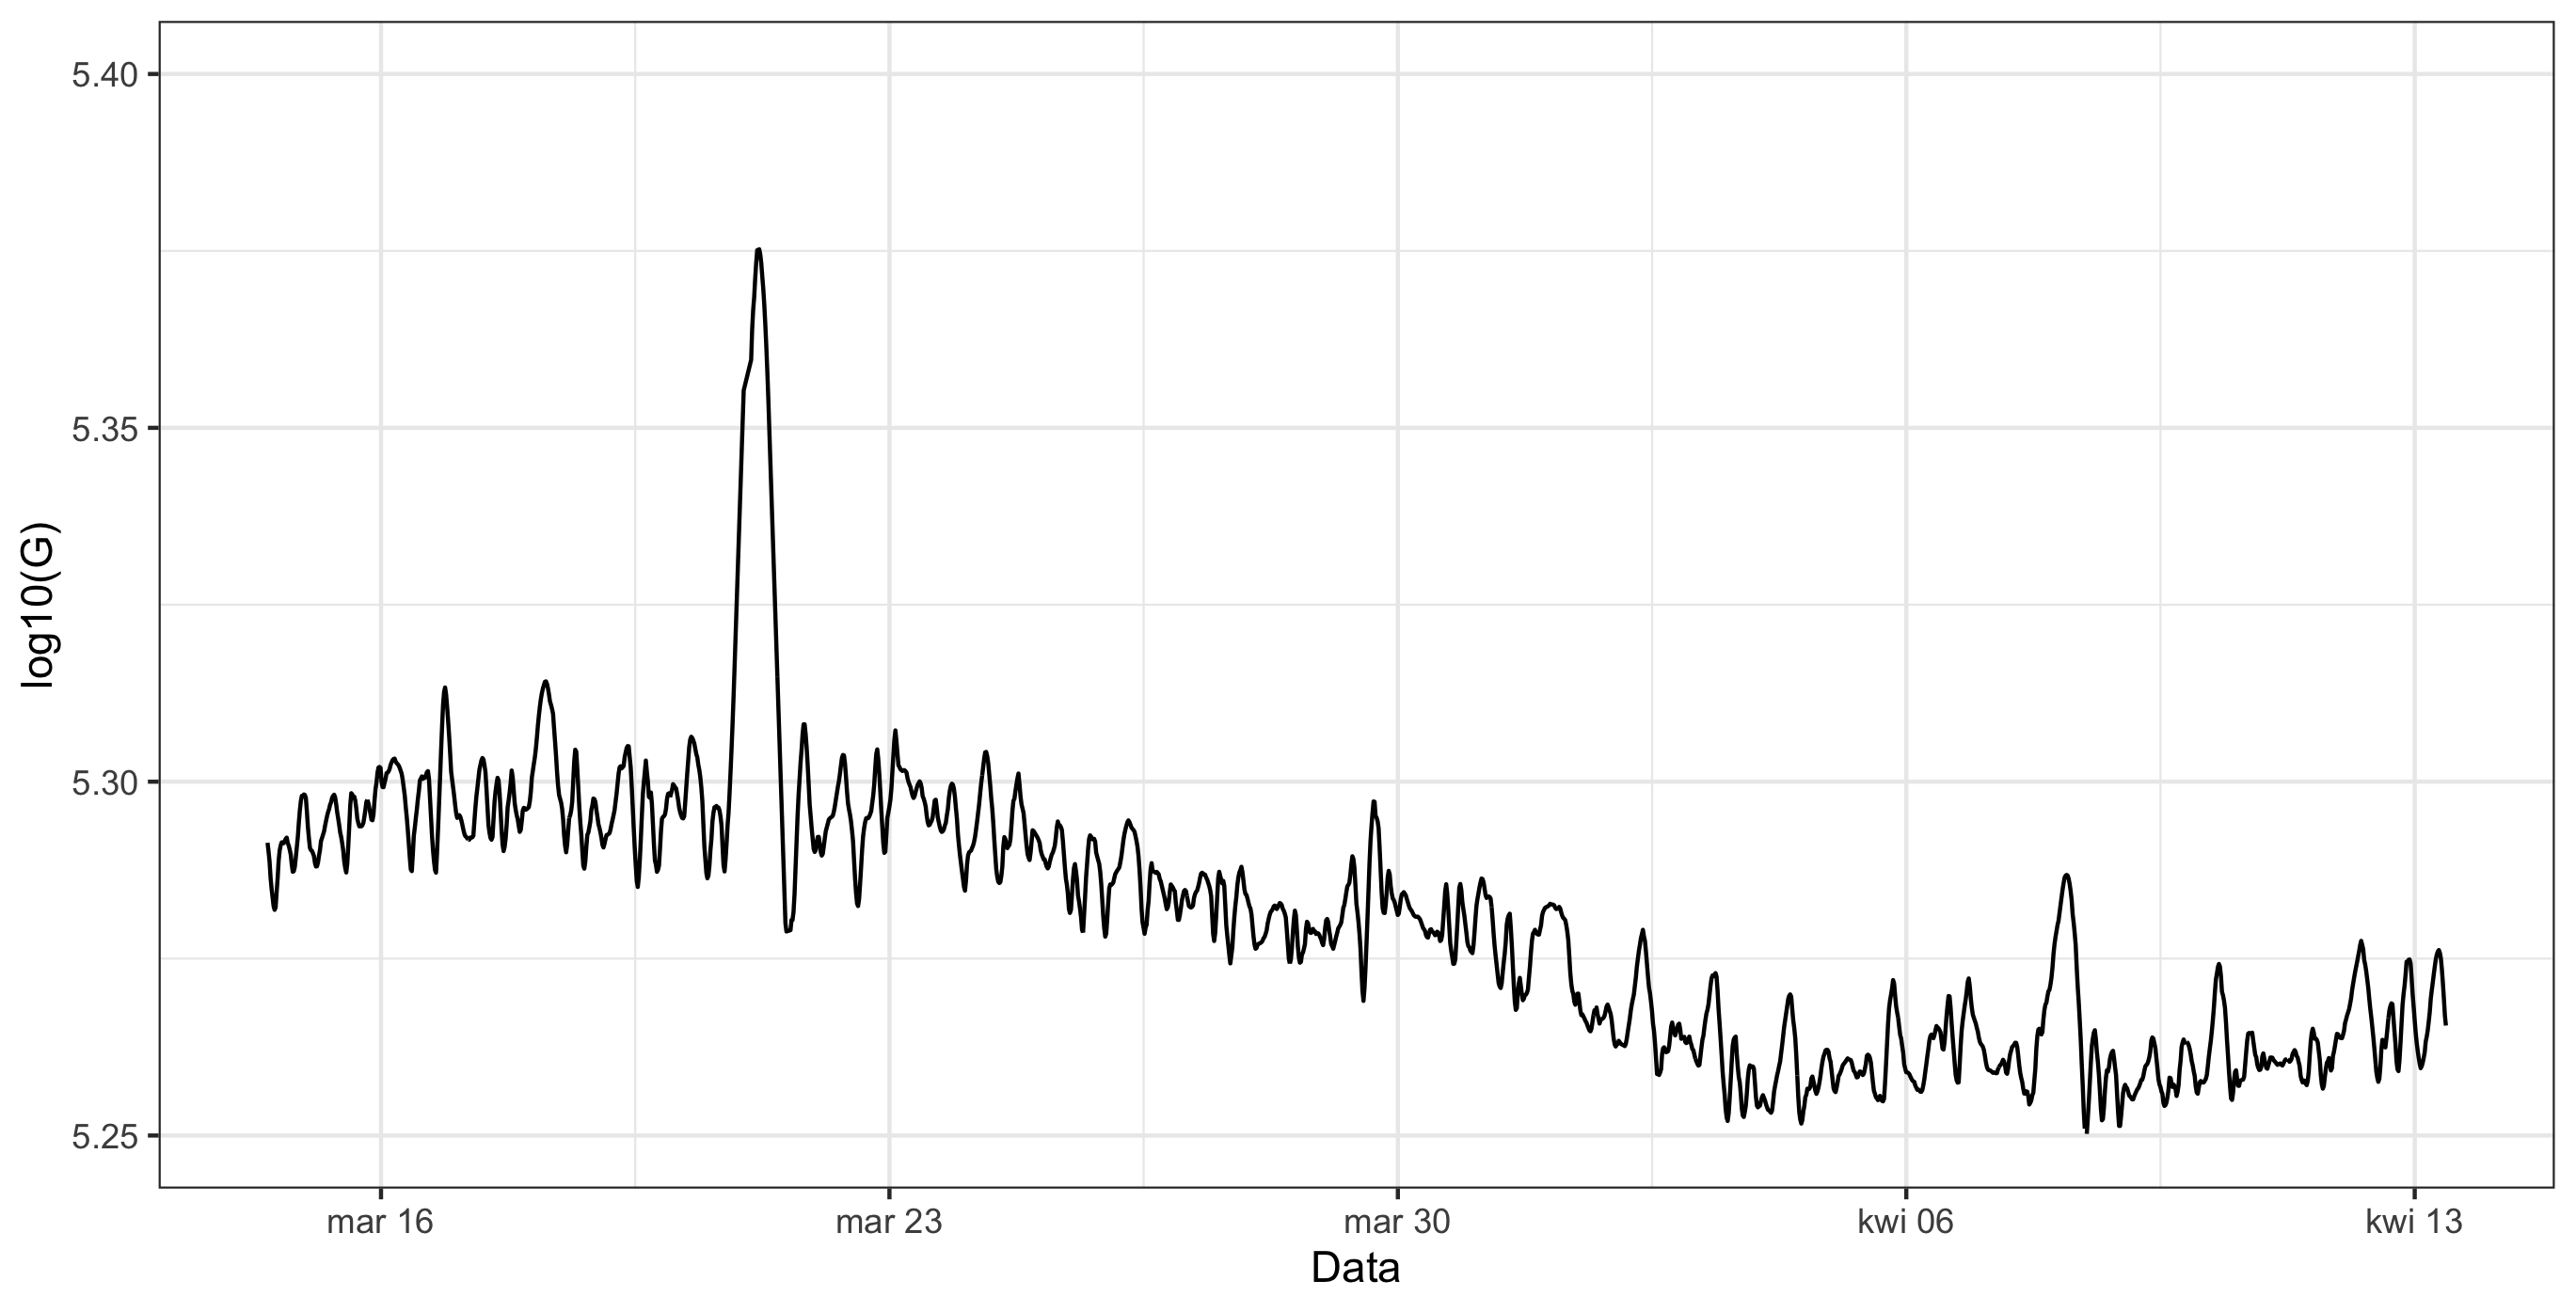
\includegraphics[width=\textwidth]{./images/wtoken-random.png}
  \caption{Przebieg wartości WoW tokna. Rysunek własny.}
\end{figure}

\section{Zadanie detekcji anomalii \label{r3}}

W rozdziale tym zostanie zdefiniowany w ogólny sposób problem detekcji
anomalii w szeregach czasowych. Konkretyzacja ogólnych pojęć
zdefiniowanych poniżej zostanie przedstawiona w rozdziale dotyczącym
algorytmów detekcji.

Przez zadanie detekcji anomalii w trakcie realizacji projektu będziemy
rozumieć następujący problem:

\begin{description}
\item[Szereg czasowy]
niech \((X_{i})_{i \in T}\) będzie procesem stochastycznym określonym na
pewnej przestrzeni probabilistycznej, a zbiór indeksów \(T\) będzie
interpretowany jako zbiór chwil czasowych jednakowo odległych od siebie.
Realizację tego procesu, tj. uporządkowany zbiór
\(\{x{_t}\}_{t = 1, \dots, N}\), będziemy nazywać szeregiem czasowym.
Nie zakładamy ponadto niczego względem stacjonarności tego szeregu lub
rozkładu prawdopodobieństwa, z którego jest on generowany poza faktem,
że jego nośnikiem jest zbiór liczb rzeczywistych \(\mathbb{R}\).
\item[Anomalia]
Anomalią w szeregu czasowym będziemy nazywali punkt w tym szeregu
\(x_{k}\), który według przyjętego kryterium \emph{odstaje} od
pozostałych punktów w najbliższym sąsiedztwie
\(x_{k - s}, \dots, x_{k + s}\) (anomalia lokalna) lub względem
wszystkich punktów w szeregu (anomalia globalna). Kryterium
\emph{odstawania} jest silnie zależne od kontekstu i procedury detekcji
anomalii. Często przyjmowane kryterium wygląda następująco
\cite{ad_review}:
\end{description}


\begin{equation}
  \label{eq1}
  |x_t - s(\{X_{t}\})| > \tau
\end{equation}

przy czym \(s(\star)\) jest pewną funkcją.

\begin{description}
\item[Detekcja anomalii]
Detekcją anomalii będziemy nazywali procedurę, pozwalającą wykryć w
    szeregu czasowym zbiór indeksów $T_{A}$ punktów uznawanych za anomalię:
\end{description}

\begin{equation*}
AD\colon \{X_{t}\} \rightarrow T_{A} \subset T.
\end{equation*}

\section{Algorytmy detekcji anomalii \label{r4}}

W rozdziale tym zostaną opisane algorytmy służące do detekcji anomalii,
które w ramach projektu zamierzamy zbadać. Opis ten nie będzie zawierał
dokładnego pseudokodu, a jedynie pewien formalizm matematyczny, który
pozwala zobrazować idee stojące za omawianymi metodami. Ponadto wskazane
i omówione zostaną parametry tych metod.

Omawiane metody

\hypertarget{stl-esd}{%
\subsection{STL-ESD}\label{stl-esd}}

Metoda STL (z ang. \emph{Seasonal-Trend decomposition using Loess})
opiera się na dekompozycji addytywnej szeregu czasowego na trzy składowe
w następującej formie

\begin{equation*}
x_{t} = \tau_{t} + s_{t} + r_{t},\; t = 1, \dots, N
\end{equation*}



gdzie \(x_{t}\) jest obserwowaną wartością szeregu czasowego,
\(\tau_{t}\) jest składową trendu, \(s_{t}\) składową sezonowości, a
\(r_{t}\) składową rezyduów. Dekompozycja taka jest dedykowana szeregom
czasowym z zauważalnymi wolnozmiennymi fluktuacjami sezonowości oraz
szybkozmienną składową trendu \cite{wen-gao}. Zakłada się
ponadto, że składowa rezyduów zawiera całą pozostałą informację o
szeregu czasowym -- m.in. szum. Można to sformalizować w następujący
sposób:

\begin{equation*}
  r_{t} = a_{t} + \epsilon_{t}
\end{equation*}



przy czym składowa \(\epsilon_{t}\) jest składową szumu, a \(a_{t}\)
modeluje poszukiwane anomalie w postaci nagłych przyrostów wartości
(t.zw. \emph{peak}'ów). Dekompozycja STL jest procedurą iteracyjną i
szczegółowo zostanie opisana w dokumentacji końcowej projektu. Na
potrzeby tego dokumentu należy zaznaczyć, że wynikiem dekompozycji jest
składowa \(a_{t}\), a składowa:

\begin{itemize}
\item
  szumu \(\epsilon_{t}\) jest usuwana wskutek operacji filtracji (ang.
  \emph{denoising}) przy pomocy średniej/mediany kroczącej lub
  probabilistycznemu wygładzaniu eksponencjalnego (PEWMA) \cite{PEWMA}
\item
  trendu \(\tau_{t}\) jest usuwana wskutek operacji detrendyzacji, która
  w najprostszym wariancie sprowadza się do zastosowania operatora
  różnicowego \begin{equation*} \nabla x_{t} = x_{t} - x_{t -1} \end{equation*}
    lub do filtrów kroczących
\item
  sezonowości \(s_{t}\), która jest usuwana w standardowej wersji
  metody STL przy pomocy LOESS (ang. \emph{locally estimated scatterplot
  smoothing}), tj. metody łączącej działanie średniej kroczącej z
  regresją wielomianową \cite{stl-origin}.
\end{itemize}

STL zawiera trzy parametry sterujące metodą:

\begin{enumerate}
\def\labelenumi{\arabic{enumi}.}
\item
  \(n_{p}\) liczbę obserwacji, która jest rozważana w każdym cyklu
  wyliczania składowej sezonowości
\item
  \(n_{i}\) liczbę iteracji wewnętrznej pętli algorytmu
\item
  \(n_{o}\) liczbę iteracji pętli zewnętrznej
\end{enumerate}

oraz trzy lub więcej parametrów sterujących detrendyzacją, usunięciem
szumu oraz ekstrakcją sezonowości.
%%%%%%%%%%% GESD

Po otrzymaniu składowej \(a_{t}\) stosowany jest test (ang. Generalized Extreme Studentized Deviate test), który służy do wykrycia anomalii w badanym szeregu. Test ten stopniowo dostosowuje się do badanego szeregu przez wyrzucanie najbardziej odstających wartości i ponowne obliczanie wartości krytycznej. Przez odrzucenie kolejnych wartości zawyżających  ustala się wartość krytyczna. Test ten dostosowuje się przez parametr \[\alpha\] mówiący o szerokości wartości odstających do odrzucenia oraz przez procent anomalii spodziewanych w szeregu. Jest to metoda iteracyjna przez to jest bardziej czasochłonna niż np IQR jednak jest też bardziej odporna na wpływ wysokich anomalii.   

% Po otrzymaniu składowej \(a_{t}\) stosowany jest test statystyczny ESD
% (z ang. \_Extreme Studentized Deviate), który służy do wykrycia
% anomalii w próbie o rozkładzie \emph{asymptotycznie} normalnym. Jest on
% uogólnieniem testu Grubbs'a, w którym rozkład normalny próby jest
% warunkiem koniecznym. Test ESD rozważa dwie hipotezy

% \newtheorem{nullhypothesis}{$H_0\colon$}
% \newtheorem{althypothesis}{$H_1\colon$}

% \begin{nullhypothesis}
%   w próbie \(\{a_1, \dots, a_{n}\}\) nie ma punktów odstających (anomalii) 
% \end{nullhypothesis}

% \begin{althypothesis} 
%   w próbie \(\{a_1, \dots, a_{n}\}\) jest co najwyżej \(K\) punktów odstających.
% \end{althypothesis}


% \(i\)-ta statystyka testowa ESD wyliczana jest w następujący sposób:

% \begin{equation*}
% T^{ESD}_{i} = \frac{\max_{i}|a_{i} - \bar a|}{\sigma}
% \end{equation*}

% gdzie \(\bar{a}\) oznacza średnią z próby, a \(\sigma\) odchylenie
% standardowe z próby. Po wyliczeniu \(T^{ESD}_{i}\) usuwana jest z próby
% obserwacja maksymalizująca licznik i liczona jest kolejna statystyka
% testowa na podstawie zmodyfikowanej próby.

% Po wyliczeniu \(\{T^{ESD}_{i}\}_{i = 1, \dots, K}\) wyliczane są
% wartości krytyczne testu \(\lambda_{i}\) będące funkcją rozkładu
% t-studenta z \(N - i\) stopniami swobody.

% Liczbę anomalii w próbie znajduje się przez podanie największego \(i\)
% takiego, że \(T^{ESD}_{i} > \lambda_{i}\).

% W kontekście definicji procedury detekcji anomalii podanej (\ref{r3})
% należy wybrać z próby \(i\) największych elementów i ich znaczniki
% umieścić w zbiorze \(T_{A}\).

Dekompozycja szeregu czasowego przez algorytm STL znajduje się na
poniższym obrazku.

\begin{figure}[H]
\centering
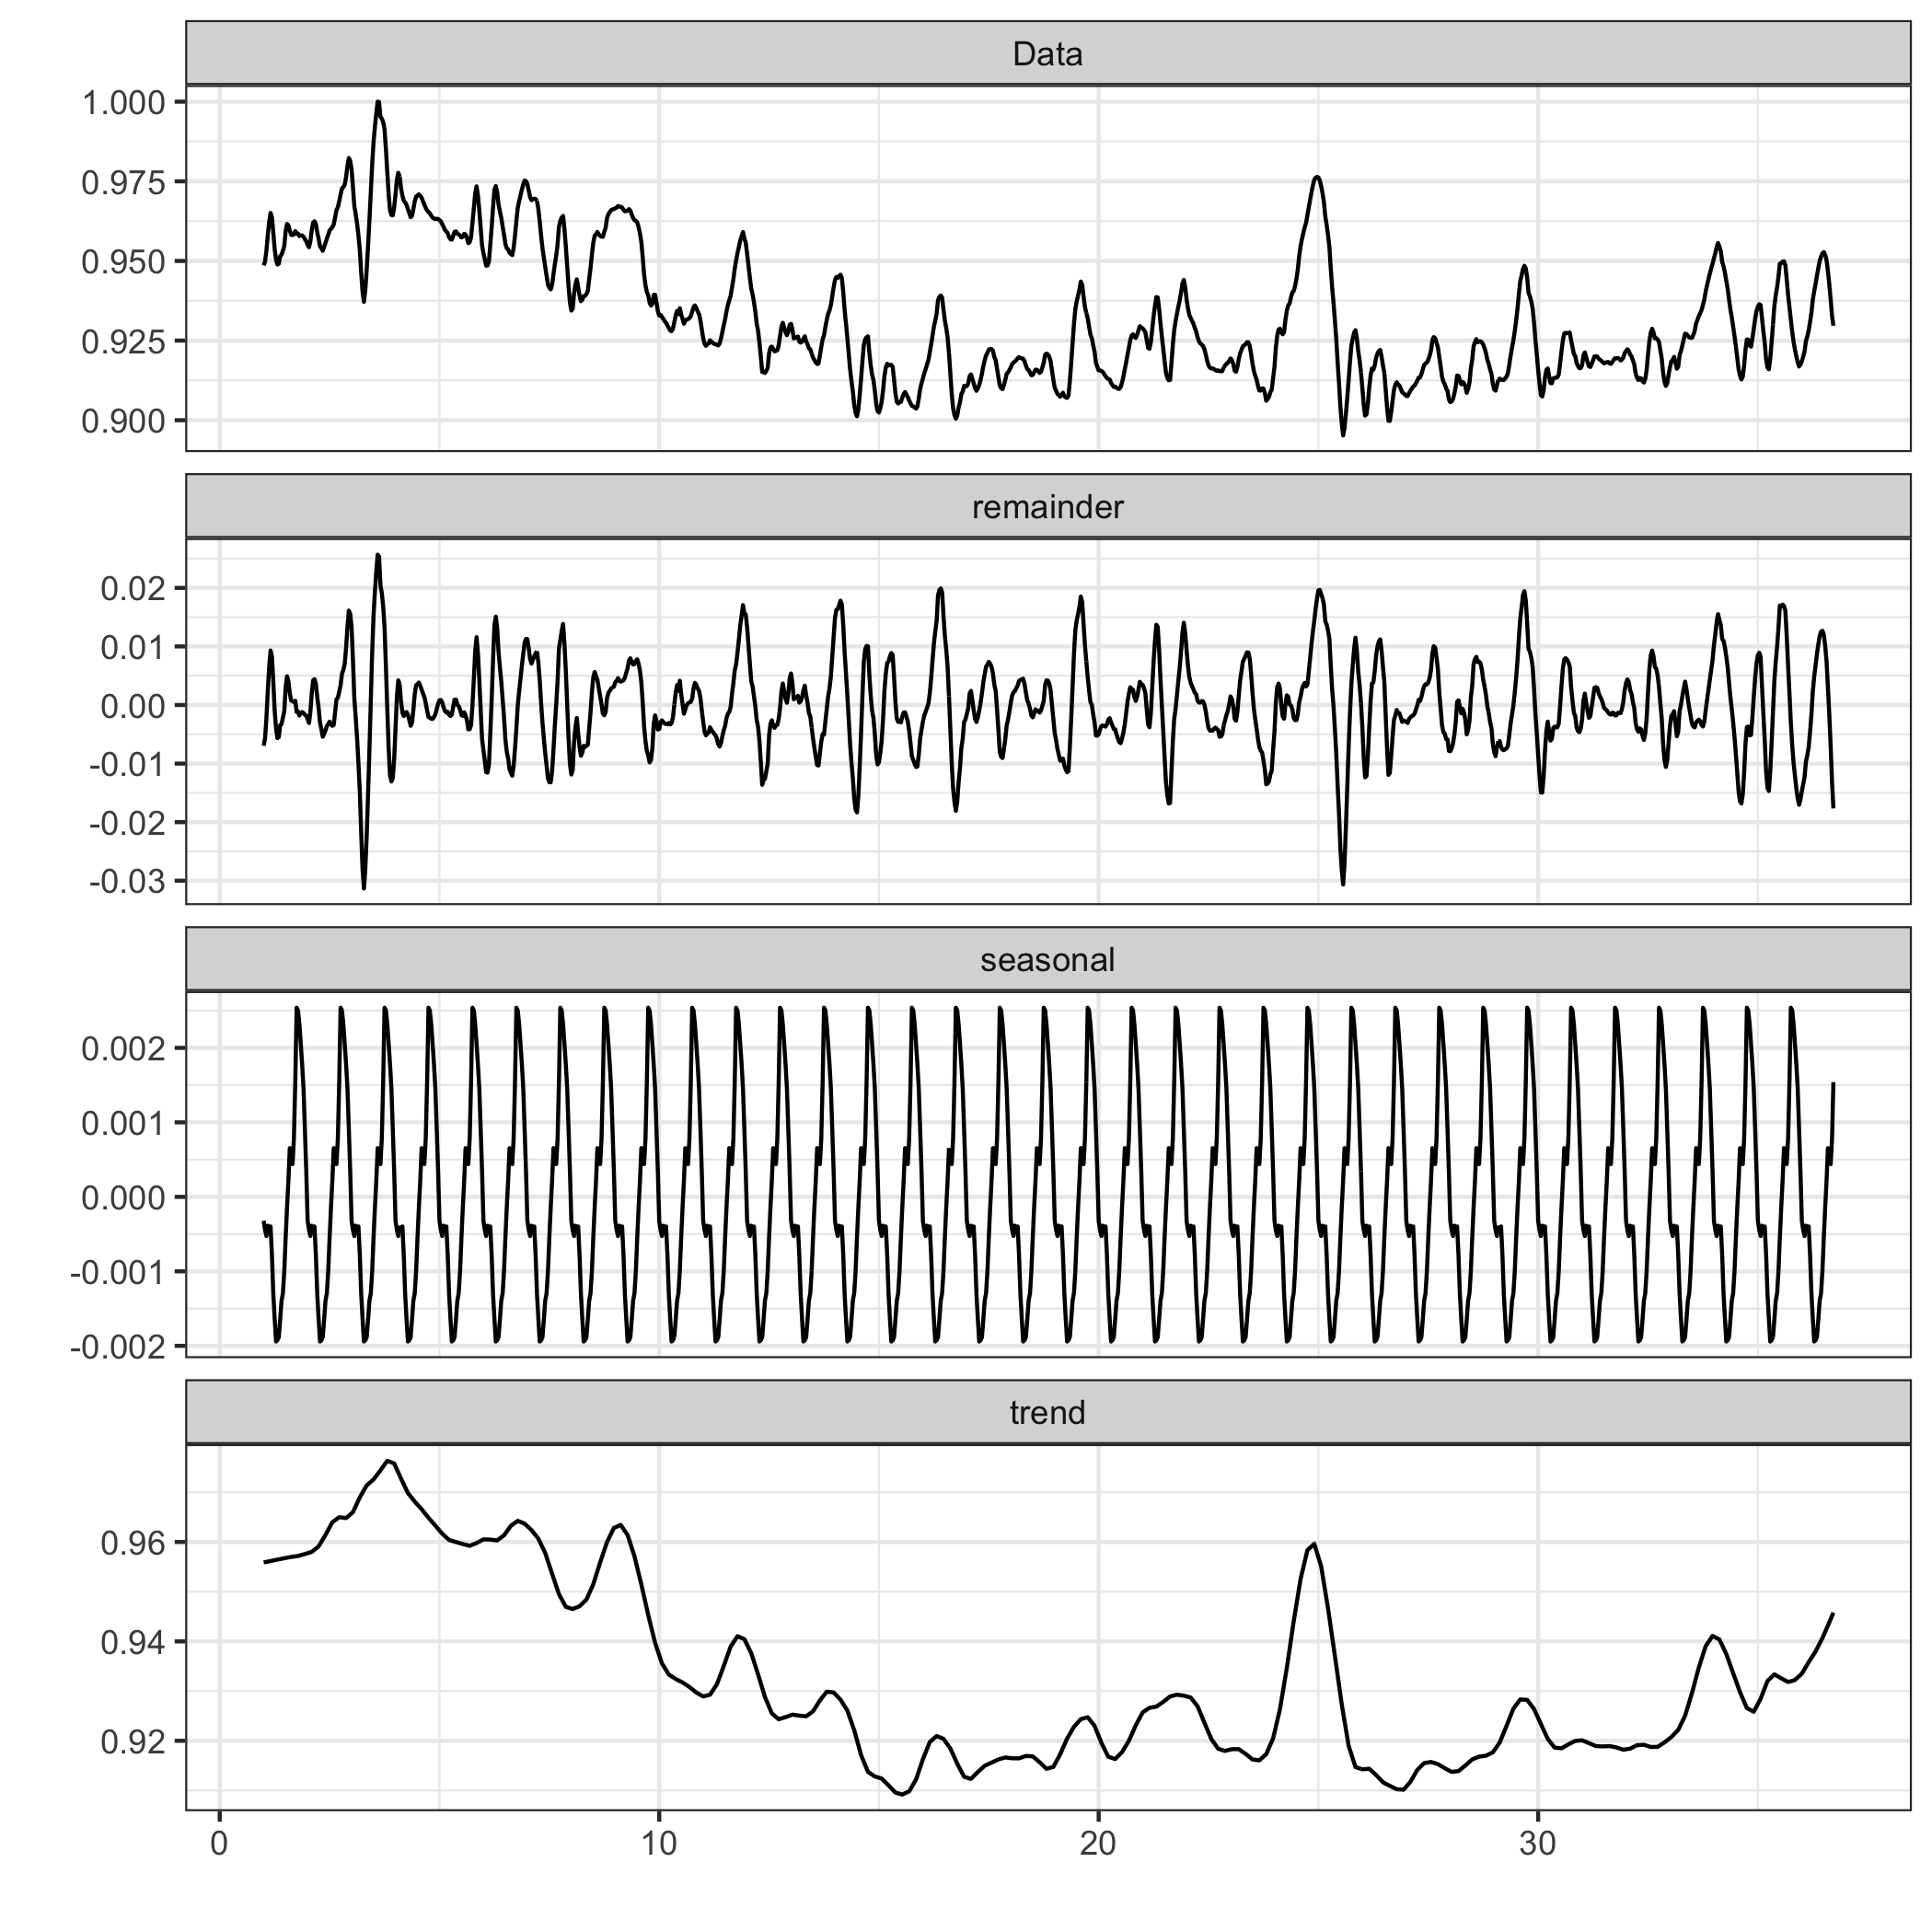
\includegraphics[width=\textwidth]{./images/stl-usage.png}
\caption{Dekompozycja szeregu czasowego metodą STL. Rysunek własny.}
\end{figure}

\subsection{Metody oparte na zanurzeniu szeregu czasowego w przestrzeni wielowymiarowej}

Algorytm bazuje na kroczącym oknie historii o długości $k$, które zanurza (ang. \emph{embed}) szereg czasowy w przestrzeni $k$-wymiarowej. Operacja taka umożliwia zastosowanie metod wielowymiarowych takich jak las izolacyjny, SVM lub LOF. Ważnym elementem występującym we wszystkich metodach tego typu jest dobór odpowiedniej wartości parametru $k$. Jeśli wartość $k$ będzie za mała algorytm będzie podatny na szum, natomiast jeśli $k$ będzie zbyt duże algorytm będzie niewrażliwy na lokalne anomalie. 

\subsubsection{Las Izolacyjny}
 Algorytm ten wybiera losową wartość podziału w przedziale między maksymalną a minimalną wartością cechy. w ten sposób dzielony jest cały zakres wartości cechy. W efekcie powstaje drzewo binarne w którym, ilość podziałów wymagana do wyizolowania próbki jest równa odległości od liścia do korzenia. Funkcją decyzyjną jest ta odległość, uśredniona względem drzew lasu. Jest ona miarą czy dana próbka jest anomalią czy nie.
  \[s(x, n) = 2^{\frac{-E(h(x)}{c(n)}}\]
  gdzie $E(h(x))$ jest uśrednioną względem wszystkich drzew długością ścieżki (ilością węzłów) prowadzącej od liścia do korzenia, $c(n)$ jest średnią długością ścieżki w drzewie, a $n$ jest ilością węzłów drzewa. \\
  Próbki będące anomaliami zwykle wymagają mniejszej ilości podziałów aby przejść z korzenia do liści. Gdy funkcja $s(x, n)$ osiąga wartości bliskie 1 to badany punkt z dużym prawdopodobieństwem jest anomalią, jeśli natomiast osiąga wartości bliskie 0.5 to punkt jest normalny.  \\
  
  Algorytm ten ma następujące parametry:
  \begin{itemize}
      \item rate Kontroluje on jaka część próbek średnio będzie uznawanych za anomalię. Przyjmuje wartości z zakresu $[0,1]$. Parametr ten zostanie dobrany eksperymentalnie. 
      \item ntrees - liczba wykorzystanych drzew 
      \item min-gain - minimalna zdobycz informacyjna konieczna żeby kontynuować podział
      \item prob-pick-avg-gain - prawdopodobieństwo podziału według atrybutu dającego największą średnia zdobycz informacyjną (wartość od 0 do 1)
      \item prob-pick-pooled-gain - prawdopodobieństwo podziału według atrybutu dającego największą łączną zdobycz informacyjną (wartość od 0 do 1) % nie wiem czy tak jest ok 
  \end{itemize}

\subsubsection{Jednoklasowy SVM}

Jednoklasowy SVM (z ang. Support Vector Machine) jest nienadzorowaną metodą detekcji anomalii. 
\begin{equation}
    min_{w \in F, \bf{\xi} \in \mathbb{R}, \rho \in \mathbb{R}}\; x\ \frac{1}{2}||w||^{2} + \frac{1}{vl}\sum_{i} \xi_{i} - \rho 
    z ograniczeniami \text{subject to}\; (w\cdot\Psi(\textbf{x}_{i})) \geq \rho - \xi_{i}, \; \xi_{i} \leq 0
\end{equation}


Na podstawie tego równania wyznaczana jest funkcja $f$, która przyjmuje wartość 1 w niewielkim obszarze obejmującym znaczną część punktów (obszar gdzie punkty mają duże zagęszczenie) i wartość -1 w pozostałym obszarze. 
Dla nowych próbek wartość $f(x)$ wyznacza się poprzez decyzję, po której stronie hiperpłaszczyzny znajduje się ta próbka. 
Zbadane zostaną następujące parametry:
\begin{itemize}
    \item kernel - radialne jądro przekształcenia (parametr gamma)
    \item nu - jest skorelowany z górną granicą liczby źle klasyfikowanych przykładów i liczbą wektorów nośnych

\end{itemize}

\subsubsection{LOF}

LOF (z ang. Local Outlier Factor) jest nienadzorowaną metodą detekcji anomalii. Dla każdego punktu wylicza ona lrd (z ang. local reachability density) w odniesianiu do punktów z jego sąsiedztwa.

\begin{equation}
    rld(p) = \frac{1}{\frac{\sum_{o \in N} reach-dist(p,o)}{|N(p)|}}
\end{equation}

gdzie $N$ jest sąsiedztwem punktu $p$. Zasięg punktu (z ang. reachability distance ) definiowany jest jako 
\begin{equation}
    reach-dist(p,o) = max(k-dist(o), d(p,o))
\end{equation}

gdzie $d(p, o)$ to odległość między punktami $p$ i $o$, a $k-dist$ jest to odległość między punktem $o$ a jego $k$-tym sąsiadem. Wartość ta mówi o tym jak daleko znajduje się punkt od kolejnego punktu w obszarze. Im mniejsza jest ta wartość tym większa odległość między punktami. 


Następnie na podstawie lrd danego punktu i wyników uzyskanych dla jego sąsiadów obliczany jest LOF 

\begin{equation}
    LOF(p) = \frac{\sum_{o \in N} \frac{lrd(o)}{lrd(p)}}{|N(p)|}
\end{equation}. 

Za anomalię uznawany jest punkt, którego zasięg jest znacznie mniejszy od zasięgów punktów sąsiedztwa. Ma to przełożenie na współczynnik LOF - dla punktów nieodstających uśrednione zasięgi dają wartości bliskie są 1 natomiast dla anomalii wartość ta jest znacznie większa od 1.  

Wybrany musi być próg \emph{tresh} od którego wartość zostanie uznana za anomalię oraz rozmiar okna \emph{k} w jakim anomalie będą badane. 

\section{Charakterystyka zbiorów danych \label{r5}}

\subsection{WIG20}

Historyczne dane \texttt{WIG20} dostępne są do pobrania ze strony
\href{https://stooq.pl/q/d/?s=wig20}{stooq.pl} z interwałem:

\begin{itemize}
\item
  dziennym
\item
  tygodniowym
\item
  miesięcznym
\item
  kwartalnym
\item
  rocznym.
\end{itemize}

Dane pobierane są w formacie \texttt{CSV} i nie zawierają wartości
brakujących. Struktura zbioru danych przedstawiona jest na poniższym
obrazku.

\begin{figure}[H]
  \centering
  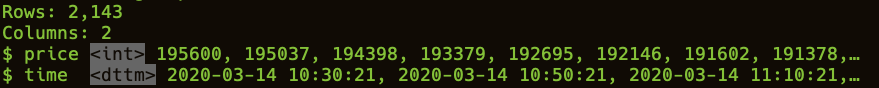
\includegraphics[width=.75\textwidth]{./images/wt-glimpse.png}
  \caption{Wynik wypisania na konsolę fragmentu zbioru danych.}
\end{figure}

Należy jednak zaznaczyć, że rozważaną w projekcie wartością szeregu
czasowego jest uśredniona wartość indeksu z wartości otwarcia,
zamknięcia oraz wartości najmniejszej i największej danej sesji.

Wartości indeksu WIG20 dostępne są od 16 kwietnia 1991 do dnia
dzisiejszego (02.04.2020) z tą uwagą, że nie we wszystkich przypadkach
zachowany jest wymagany interwał, co jest zaznaczone na rysunku poniżej.

\begin{figure}[H]
  \centering
  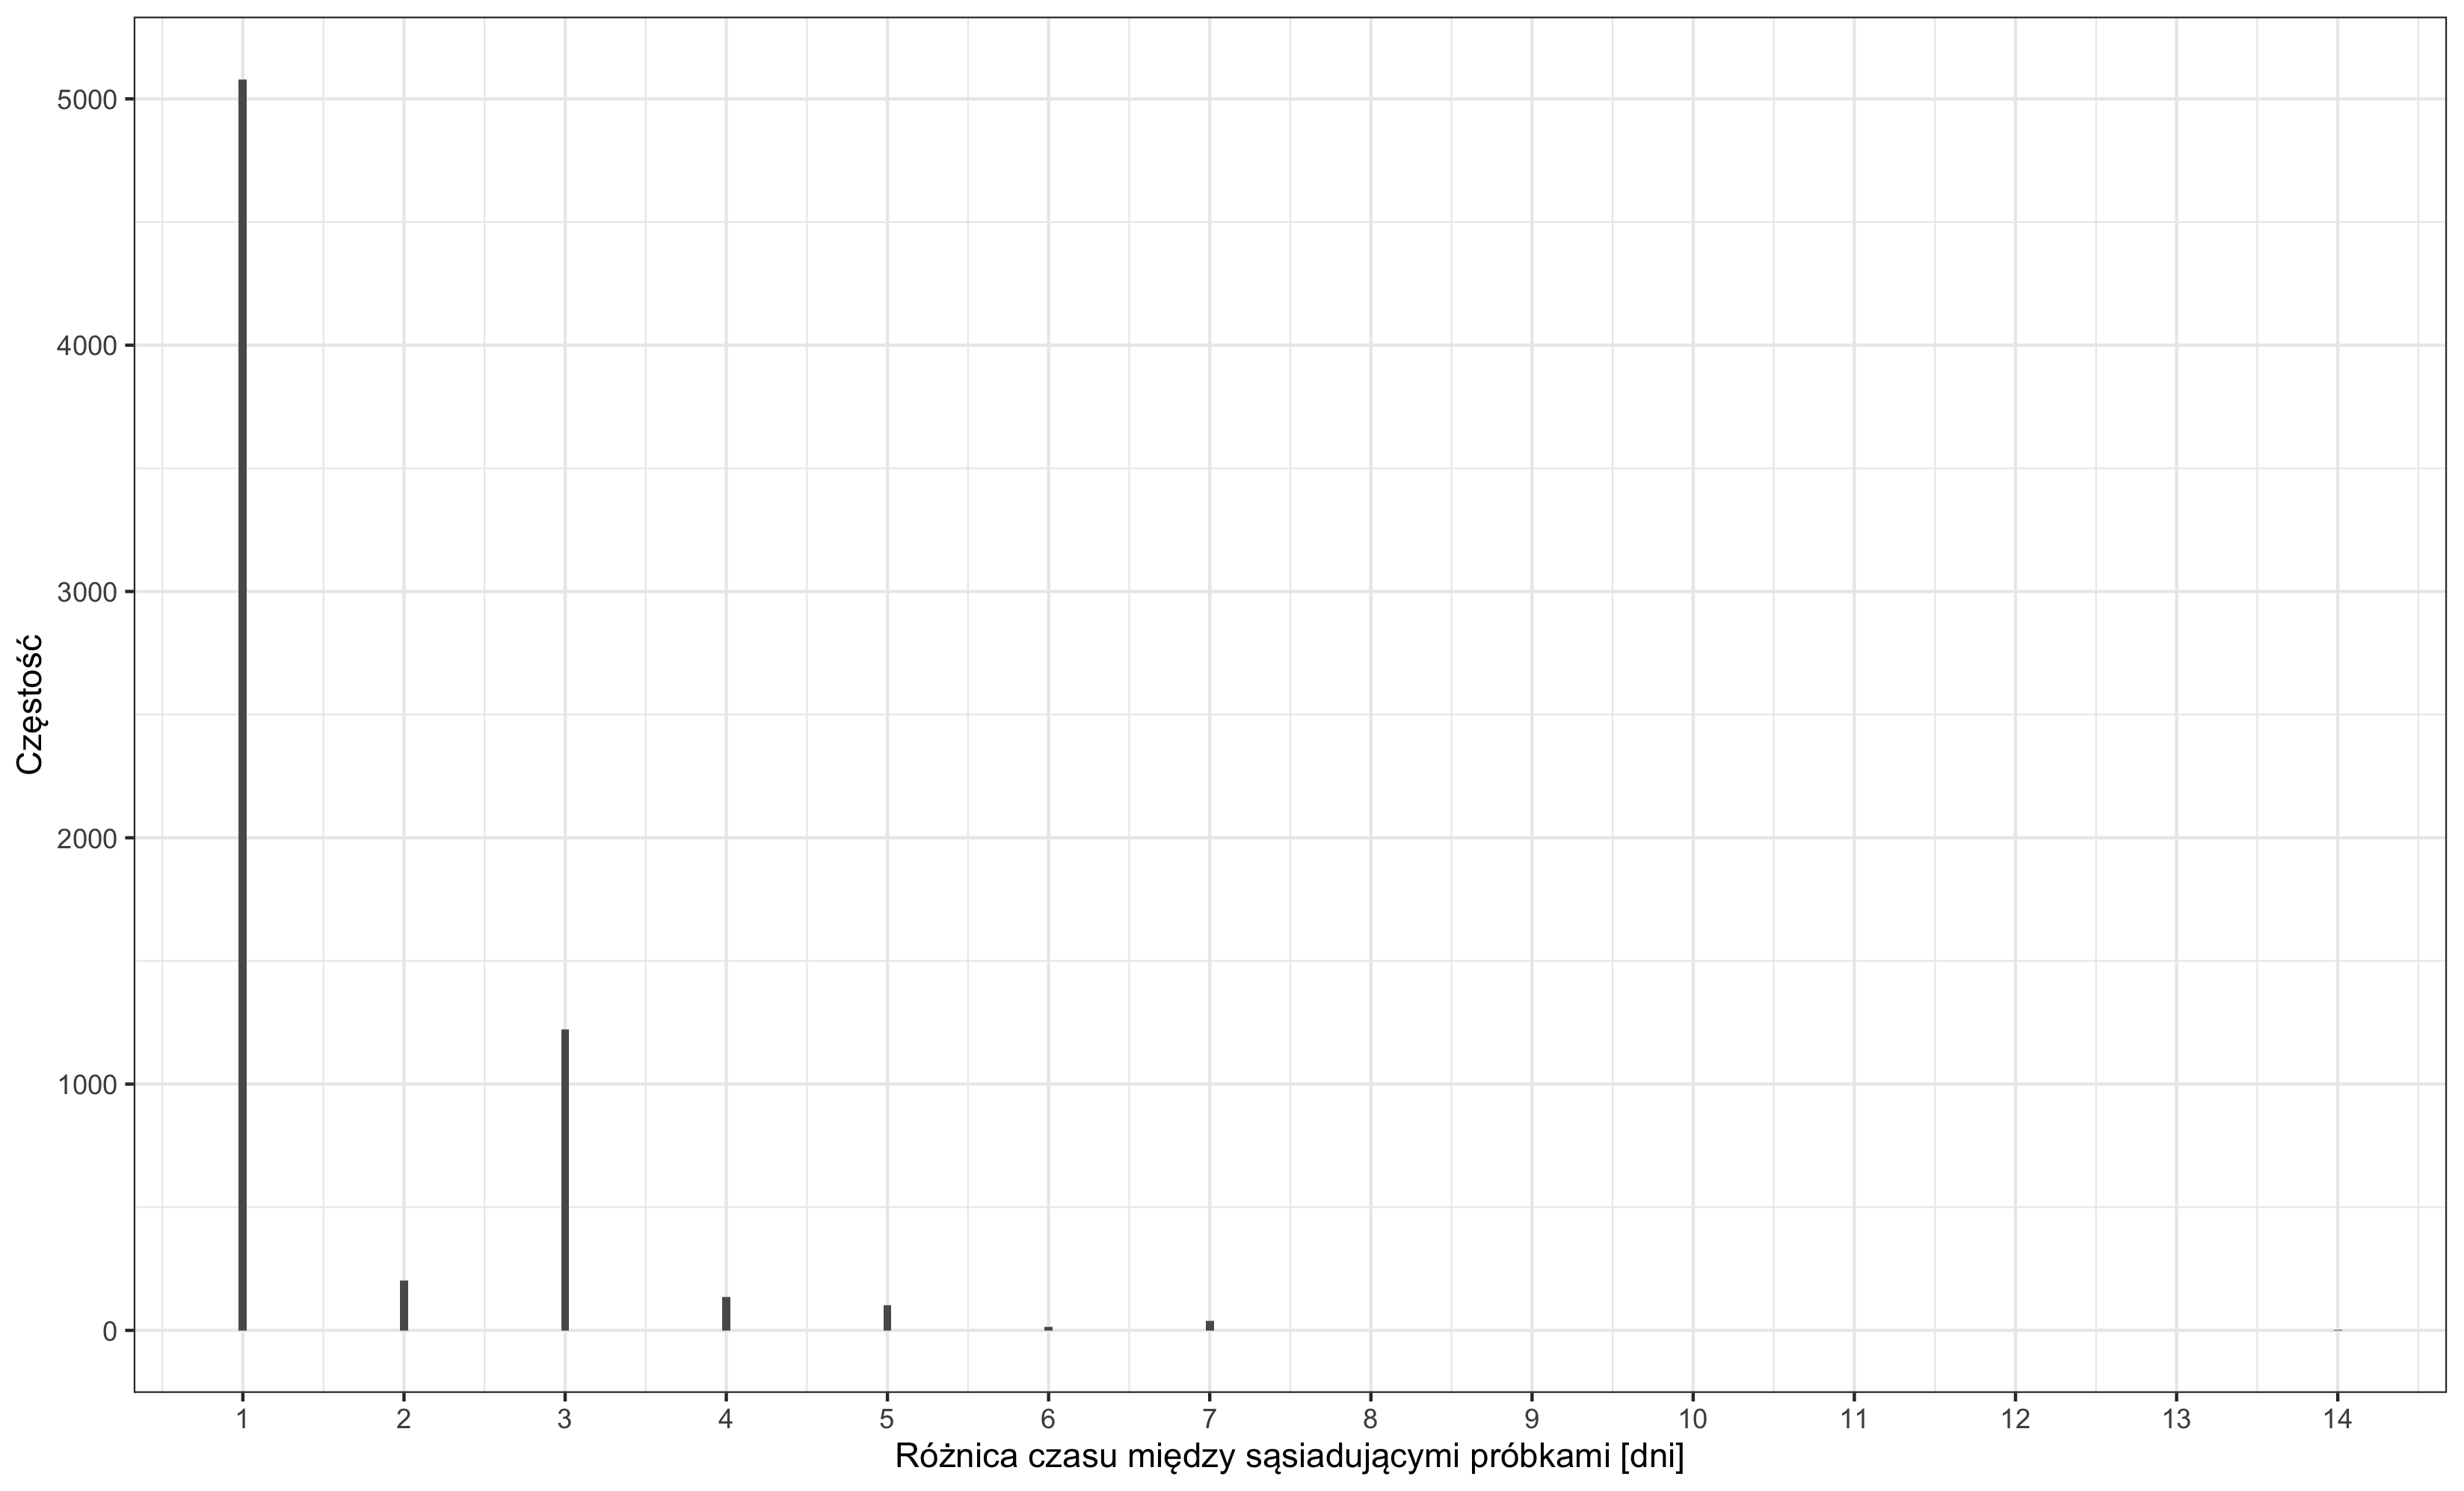
\includegraphics[width=.75\textwidth]{./images/tdiff.png}
  \caption{Histogram odstępów między sąsiadującymi próbkami w zbiorze danych WIG20. Rysunek własny.}
\end{figure}

Do badań wykorzystane zostaną dane od 1 stycznia do 16 maja 2020. Jest to 136 punktów a okres próbkowania wynosi 1 dzień.   
Poniżej przedstawione są wartość średnia, maksymalna i minimalna oraz odchylenie standardowe przebiegu. 

\begin{table}[H]
\begin{tabular}{|l|l|l|l|}
\hline
minimum & średnia & maksimum & \begin{tabular}[c]{@{}l@{}}odchylenie \\ standardowe\end{tabular} \\ \hline
4283.   & 5880.   & 7110.    & 922.                                                              \\ \hline
\end{tabular}
\end{table}

Test $\chi^2$ pozwala na stwierdzenie że dane nie mają rozkładu normalnego.  Na podstawie histogramu można zauważyć że w danych pojawia się "stopień" - występują 2 zakresy danych o rozkładach zbliżonych do normalnego. 

Na podstawie dekompozycji STL wyznaczona została składowa trendu wynosząca $trend = 67.5 dni$ oraz składowa sezonowości $T = 7 dni$

Na podstawie testu Spearmana można odrzucić hipotezę o autokorelacji szeregu. 

Poniżej przedstawione są wartości indeksu Hursta. 
\begin{table}[H]
\begin{tabular}{|l|l|}
\hline
Simple R/S Hurst estimation:        & 0.8443221 \\ \hline
Corrected R over S Hurst exponent:  & 1.0584    \\ \hline
Empirical Hurst exponent:           & 0.7784533 \\ \hline
Corrected empirical Hurst exponent: & 0.7884377 \\ \hline
Theoretical Hurst exponent:         & 0.5259013 \\ \hline
\end{tabular}
\end{table}

\hypertarget{wow-token}{%
\subsection{WoW Token}\label{wow-token}}

Historyczne kursy tokena dostępne są na stronie
\href{https://wowtokenprices.com/}{wowtokenprices.com}. Serwis
udostępnia API, które umożliwia pobrania danych z kwantem 20-minutowym,
które nie zawierają wartości brakujących, od początku istnienia tokena,
tj. od roku 2015. Kurs tokena różni się między regionami, w których
znajdują się serwery. Dostępnych jest 5 regionów, tj.

\begin{enumerate}
\def\labelenumi{\arabic{enumi}.}
\item
  europejski
\item
  amerykański
\item
  chiński
\item
  tajwański
\item
  koreański.
\end{enumerate}

Struktura zbioru danych z ostatniego miesiąca widoczna jest na na
poniższym obrazku.

\begin{figure}[H]
  \centering
  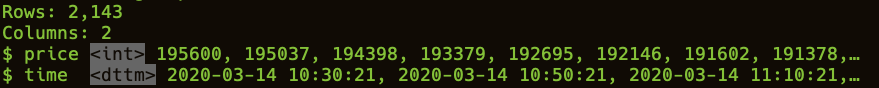
\includegraphics[width=.75\textwidth]{./images/wt-glimpse.png}
  \caption{Wynik wypisania na konsolę fragmentu zbioru danych.}
\end{figure}

Do badania wykorzystane zostaną dane od 14 marca do 13 kwietnia 2020. Jest to 2143 punkty danych próbkowane co 20 minut.  
W danych znajduje się 9 punktów odstających. Rozkład tych danych daleki jest od normalnego co potwierdza \[p_{value}<2.16*10^{-16}\] oraz histogram. Na podstawie analizy STL ustalono że trend wynosi $trend = 548.5 min$ a sezonowość ma częstotliwość $f = 72 min$. Przeprowadzony został również test autokorelacji Spearmana. Na jego podstawie można odrzucić hipotezę o autokorelacji szeregu. 


Wartości średnia, maksymalna i minimalna oraz odchylenie standardowe przebiegu przedstawione są poniżej: 
\begin{table}[H]
\begin{tabular}{|c|l|c|c|c|}
\hline
\multicolumn{2}{|c|}{Minimum}                 & \begin{tabular}[c]{@{}c@{}}wartość\\  średnia\end{tabular} & maksimum                & \begin{tabular}[c]{@{}c@{}}odchylenie\\ standardowe\end{tabular} \\ \hline
\multicolumn{2}{|c|}{\multirow{177477}} & \multirow{190819}                                    & \multirow{237263} & \multirow{8248}                                            \\
\multicolumn{2}{|c|}{}                        &                                                            &                         &                                                                  \\
\multicolumn{2}{|c|}{}                        &                                                            &                         &                                                                  \\ \hline
\end{tabular}
\end{table}

Wartości indeksu Hursta. 
\begin{table}[H]
\begin{tabular}{|c|c|}
\hline
Simple R/S Hurst estimation        & 0.8745215 \\ \hline
Corrected R over S Hurst exponent  & 0.9541106 \\ \hline
Empirical Hurst exponent           & 0.9140136 \\ \hline
Corrected empirical Hurst exponent & 0.8956772 \\ \hline
Theoretical Hurst exponent         & 0.5336546 \\ \hline
\end{tabular}
\end{table}

\section{Opis Eksperymentów \label{r6}}

Celem projektu jest zbadanie i porównanie metod detekcji anomalii w
szeregach czasowych przy pomocy danych scharakteryzowanych we
wcześniejszych rozdziałach.

Przyjęta metodologia zakłada, że zadanie detekcji anomalii zostanie
potraktowane jak zadanie klasyfikacji binarnej. Oznacza to, że przykłady
w zbiorze danych zostaną oznaczone flagą, która informuje o tym czy dany
przykład jest anomalią czy też nie.

Zebranym danym zostały przydzielone etykiety na podstawie rzeczywistych zdarzeń które mogły spowodować przyrost lub spadek wartości indeksu/tokena. Przykładowo : 

\begin{itemize}
  \item kryzys gospodarczy z 2008 roku (ogłoszenie upadłości przez bank \emph{Lehman Brothers}) (WIG20)
\item rozpoczęcie stanu epidemicznego w Polsce w związku z pandemią SARS-CoV-2 (WIG20)
\item atak Iranu na bazy wojskowe USA na początku 2020 roku (WIG20)
\item zwiększenie współczynnika przyrostu zdobywanego doświadczenia o $100 \%$ (WoW Token)
\item wydanie nowej części gry \emph{World of Warcraft} (WoW Token).
\end{itemize}

Dodatkowo w niektórych eksperymentach wykorzystane zostaną sztucznie wprowadzane anomalie punktowe. Wprowadzane są one przez wybór losowego punktu szeregu którego wartość jest zmieniana na $v = v+3*\sigma_{T_s}*\alpha$ gdzie $\sigma_{T_s}$ to odchylenie standardowe szeregu a $\alpha \in [0,1]$ to współczynnik sterujący amplitudą anomalii.  

Dzięki takiemu podejściu możliwe będzie porównanie metod detekcji w dość
ogólnym kontekście oraz sprawdzenie jak metody radzą sobie z wykrywaniem
anomalii, które odpowiadają przełomowym zdarzeniom i mają
odzwierciedlenie na rynkach. Przyjęcie takiej metodologii podyktowane jest faktem, że w dostępnych zbiorach danych autorom nie udało się znaleźć zbioru poświęconemu aktywom giełdowym.

Porównanie modeli odbędzie się przy pomocy trzech miar:

\begin{enumerate}
\def\labelenumi{\arabic{enumi}.}
\item
  precyzji 
    \begin{equation*}
       P = \frac{|S \cap G|}{|S|}
    \end{equation*}
\item
  odzysku (z ang. \emph{recall}) 
    \begin{equation*}
      R = \frac{|S \cap G|}{|G|}
    \end{equation*}

\item
  miary $F-1$
    \begin{equation*}
    F = 2\frac{PR}{P + R}
    \end{equation*}
  będącej średnią harmoniczną \(P\) i \(R\)
\end{enumerate}

przy czym \(S\) jest zbiorem poprawnie rozpoznanych anomalii, a \(G\)
jest zbiorem wszystkich anomalii w zbiorze danych.


\section{Eksperymenty}
Zdecydowano się na zastosowanie nienachodzących na siebie okien przetwarzania aby uniknąć wielokrotnej detekcji tej samej anomalii. Rozwiązanie to jednak może powodować zmniejszenie liczby znajdowanych anomalii. Każdy z algorytmów przetestowany zostały na dwóch zbiorach danych. Zawierają one 2 rodzaje anomalii - anomalie punktowe wprowadzane sztucznie oraz anomalie prawdziwe. 

\subsection{LOF}
W pierwszym eksperymencie sprawdzony został wpływ rozmiaru okna zanurzającego szereg czasowy na poprawność detekcji przy stałych parametrach modelu. Dobrana na tej podstawie została wartość k = ... dla której przeprowadzone były kolejne eksperymenty. 

Następnym eksperymentem było zbadanie zależności liczby sąsiadów branych pod uwagę od poprawności detekcji. 

Algorytm ten dobrze radzi sobie z anomaliami w postaci szpilek jednak anomalie przedziałowe wykrywane są gorzej. 


\subsection{Jednoklasowy SVM}
W pierwszym eksperymencie sprawdzony został wpływ rozmiaru okna zanurzającego szereg czasowy na poprawność detekcji przy stałych parametrach modelu. 

Gotowa metoda udostępniona w bibliotekach R oferuje tylko możliwość zwracania wartości TRUE i FALSE w zależności od tego czy jest uznana za anomalię dla poszczególnych przetwarzanych punktów. Oznacza to konieczność dobrania progu uznania za anomalię, został on ustalony na ... co jest przybliżonym ułamkiem anomalii w danych. 

Przy badaniu tego modelu skupiono się na jądrze radialnym, zmieniany był parametr gamma w w zakresie 0.001 do 0.05. 

Zbadany został też wpływ parametru nu skorelowanego z liczbą wektorów nośnych na jakość klasyfikacji. Zmieniany był on w zakresie od 0 do 1. Parametr ten wpływa też na liczbę wykrywanych anomalii.   

\subsection{STL}
Zastosowanie tej metody nie wymaga wstępnego zanurzania szeregu czasowego w przestrzeni wielowymiarowej. Do wyznaczenia progu anomalii na sygnale reszty wykorzystana została funkcja GESD.

Zbadany został rozmiar okna s.window wykorzystywanego do ekstrakcji sezonowości. Znalezione zostało okno o optymalnym rozmiarze s.window = 217. Oznacza to, że w szeregu czasowym pojawia się sezonowość o podobnym trwaniu.   

Zbadany został wpływ liczby iteracji pętli wewnętrznej algorytmu w zakresie od 1 do 5. Zaobserwowano, że wyniki są znacznie lepsze dla małej liczby iteracji - rzędu 1, 2. Pętla ta odpowiada za ekstrakcję składowej trendu. Większe powodują nadmierne wygładzenie sygnału a w efekcie utratę anomalii. 

Zbadany został wpływ liczby iteracji pętli zewnętrznej algorytmu w zakresie od 0 do 5. Wartość tego parametru ma znaczny wpływ na liczbę wykrywanych anomalii. Im więcej iteracji tym większe jest wygładzenie sygnału a tym samym więcej anomalii jest traconych. Do tego zadania najlepiej wykorzystać wartość 0. 

Algorytm ten bardzo dobrze odnajduje sztuczne anomalie mające postać bardzo cienkiej szpilki - pojedynczych punktów o znacznie wyższej wartości. Dobrze radzi sobie też z anomalią przedziałową o dużej amplitudzie. Pojawia się jednak problem z anomaliami o niższej amplitudzie, które giną w otoczeniu większych. Mogą też one ulegać zbyt dużemu wygładzeniu przy ekstrakcji składowej trendu i sezonowości.Zarówno anomalie punktowe jak i przedziałowe o niższych amplitudach nie są wykrywane. Jednak przyglądając się składowej reszty można je zauważyć. Nie są one jednak uznawane za anomalie przez ustalenie wartość progu. Jeśli jednak wartość progu ustawi się niżej bardzo dużo próbek zostanie uznanych za odstające. 

Wraz zwiększaniem liczby sztucznych wprowadzanych anomalii zmniejsza się liczba anomalii wykrywanych. Powodowane jest to wzrostem średniej wartości sygnału reszty a zatem niższe anomalie nie są znajdowane gdyż ich wartości znajdują się pod progiem. 

\subsection{Las izolacyjny}

W pierwszym eksperymencie sprawdzony został wpływ rozmiaru okna zanurzającego szereg czasowy na poprawność detekcji przy stałych parametrach modelu. 

Kolejnym eksperymentem było zbadanie wpływu ilości drzew na jakość detekcji. Zbadane zostały liczby drzew od 50 do 900. 

Zwiększanie liczby drzew powoduje poprawę jakości klasyfikacji tylko do pewnego momentu, przy ntrees = ... osiągane jest maksimum. Dalsze zwiększanie ich liczby powoduje pogorszenie jakości klasyfikacji.  

Badanie wpływu minimalnej zdobyczy informacyjnej wymaganej aby kontynuować podział. Parametr ten wpływa na głębokość tworzonych drzew, im jest większy tym mniej rozgałęzień będą miały drzewa. Zbadany został zakres parametru od 0 do ?? 

Prawdopodobieństwo wyboru parametru podziału według średniej zdobyczy informacyjnej mówi o tym jak często wybór parametru podziału będzie losowy a jak często podyktowany będzie zdobyczą informacyjną. Im jest on większy tym rzadziej parametr podziału wybierany jest losowo. Zmieniany był on w zakresie od 0 do 1.

Prawdopodobieństwo wyboru parametru podziału według łącznej zdobyczy informacyjnej mówi o tym jak często wybór parametru podziału będzie losowy a jak często podyktowany będzie zdobyczą informacyjną. Im jest on większy tym rzadziej parametr podziału wybierany jest losowo. Zmieniany był on w zakresie od 0 do 1.

\section{Podsumowanie}
Detekcja anomalii w danych giełdowych jest skomplikowanym zadaniem. Niewiele jest dostępnych oznaczonych zbiorów danych przygotowanych do tego zadania. Podczas etykietowania pojawia się problem jednoznacznego stwierdzenie co jest anomalią w takim przebiegu. Prostszym zadaniem jest odnalezienie anomalii na rynku wirtualnym gdyż zazwyczaj wynikają one z pojedynczych wydarzeń w świecie gry.  

W zadaniu tym problem stanowi niewielki procent danych klasyfikowanych jako anomalie w zbiorze. Zwykle zadanie klasyfikacji wymaga zrównoważonej liczby klas.  

Znacznie lepiej odnajdowane są anomalie w postaci szpilek niż przedziałów. Nie jest to jednak dokładne odwzorowanie rzeczywistego wyglądu anomalii. Zwykle w przypadku danych giełdowych anomalie takie trwają przez kilka próbek. 

Najlepszą metodą do detekcji anomalii okazał się ... 
Najgorszą natomiast okazała się ...

Wadą metody STL jest założenie, że dane są sezonowe co wprowadza ograniczenie w możliwych zastosowaniach. Nie posiadają jej inne metody, które można zastosować nie wprowadzając założeń o rozkładzie i przebiegu danych . 

Metoda LOF wykonuje się stosunkowo długo w porównaniu z innymi.
\bibliography{biblio} 
\bibliographystyle{ieeetr}
\end{document}t
